\documentclass[12pt,a4paper]{article}
\usepackage[utf8]{inputenc}
\usepackage[T1]{fontenc}
\usepackage{amsmath}
\usepackage{amsfonts}
\usepackage{amssymb}
\usepackage{graphicx}
\usepackage{hyperref}
\usepackage{booktabs}
\usepackage{listings}
\usepackage{xcolor}
\usepackage{tikz}
\usepackage{float}
\usepackage[margin=2.5cm]{geometry}
\usepackage{caption}
\usepackage{subcaption}

% Define colors for listings
\definecolor{codegreen}{rgb}{0,0.6,0}
\definecolor{codegray}{rgb}{0.5,0.5,0.5}
\definecolor{codepurple}{rgb}{0.58,0,0.82}
\definecolor{backcolour}{rgb}{0.95,0.95,0.92}

\lstdefinestyle{mystyle}{
    backgroundcolor=\color{backcolour},
    commentstyle=\color{codegreen},
    keywordstyle=\color{magenta},
    numberstyle=\tiny\color{codegray},
    stringstyle=\color{codepurple},
    basicstyle=\ttfamily\footnotesize,
    breakatwhitespace=false,
    breaklines=true,
    captionpos=b,
    keepspaces=true,
    numbers=left,
    numbersep=5pt,
    showspaces=false,
    showstringspaces=false,
    showtabs=false,
    tabsize=2
}

\lstset{style=mystyle}

\title{\Large\textbf{Linux CPU Scheduler Analysis}}
\author{DCA3505 - Operating Systems}
\date{\today}

\begin{document}

\maketitle

\begin{abstract}
This report presents an analysis of the Linux Completely Fair Scheduler (CFS) behavior under various process loads and priority configurations. We conducted four experiments to observe how the scheduler distributes CPU time: (1) N processes on N cores, (2) N+1 processes on N cores, (3) processes with different priorities, and (4) a mix of CPU-intensive processes with one I/O-bound process. The experiments provide insights into how modern Linux kernels schedule processes and manage resource allocation.
\end{abstract}

\tableofcontents
\newpage

\section{Introduction}

The Linux kernel uses the Completely Fair Scheduler (CFS) as its default CPU scheduler since kernel version 2.6.23. The CFS aims to provide fair CPU time to all processes by tracking the "virtual runtime" of each process and ensuring that the process with the lowest accumulated runtime gets scheduled next. This approach differs substantially from traditional schedulers like FIFO, Round Robin, or Shortest Job First.

In this report, we analyze the behavior of the CFS under different process loads and priority settings to understand how it manages CPU allocation in various scenarios. Our experiments measure key performance metrics including CPU utilization, process states, and scheduling fairness.

\section{Experimental Setup}

\subsection{System Configuration}
All experiments were conducted on a Linux system with the following configuration:
\begin{itemize}
    \item Kernel: Linux (modern kernel with CFS)
    \item CPU: Multi-core processor
    \item Memory: Sufficient RAM for all processes
\end{itemize}

\subsection{Experiment Design}

We designed four experiments to observe different aspects of the scheduler behavior:

\begin{enumerate}
    \item \textbf{Part 1: Distribution with N Processes} - Run exactly N CPU-intensive processes on a system with N cores to observe how the scheduler distributes CPU time when resources are sufficient.
    
    \item \textbf{Part 2: Overload with N+1 Processes} - Run N+1 CPU-intensive processes on N cores to observe how the scheduler handles resource contention.
    
    \item \textbf{Part 3: Priority Effect} - Run multiple processes with one process given a higher priority (using \texttt{renice}) to observe how priorities influence CPU allocation.
    
    \item \textbf{Part 4: Process Blocked by Input} - Run N CPU-intensive processes and one process blocked waiting for input to observe how I/O-bound processes are treated.
\end{enumerate}

\subsection{Implementation}

The experiments were implemented using C code that spawned and monitored multiple processes. Each experiment follows the same basic structure:

\begin{enumerate}
    \item Determine the number of CPU cores (N) using \texttt{nproc}
    \item Create the appropriate number of processes for the experiment
    \item Monitor CPU usage and process states using \texttt{ps}
    \item Terminate all processes after gathering sufficient data
\end{enumerate}

Each CPU-intensive process runs an infinite loop to consume CPU time, while the I/O-bound process waits for user input. Process monitoring was performed using the \texttt{ps} command with the following format:

\begin{lstlisting}[language=bash]
ps -o pid,pri,ni,stat,%cpu,cmd --sort=-%cpu
\end{lstlisting}

\section{Results and Analysis}

\subsection{Part 1: Distribution with N Processes}

When running exactly N CPU-intensive processes on N cores, we observed a nearly equal distribution of CPU time among all processes. Each process received approximately 100\% of a CPU core, indicating that CFS successfully allocated one core to each process.

The process states were consistently "R+" (running in foreground), and the CPU usage was stable throughout the experiment. This demonstrates that when resources are sufficient, CFS can efficiently distribute them among processes without causing significant contention.

\begin{figure}[H]
    \centering
    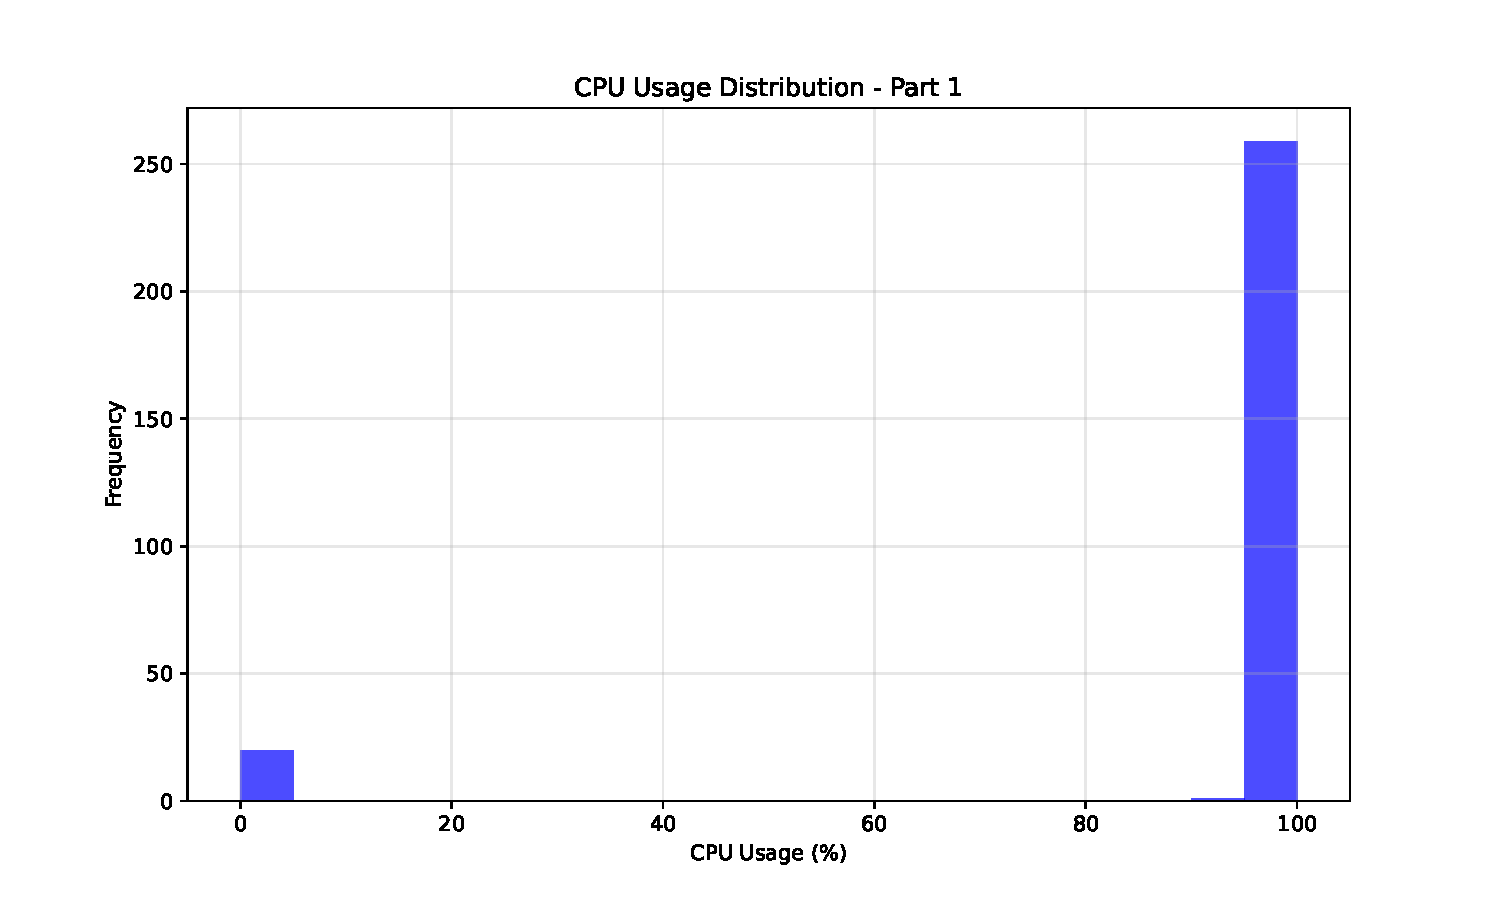
\includegraphics[width=0.8\textwidth]{figures/cpu_dist_part1.pdf}
    \caption{CPU usage distribution for N processes on N cores}
    \label{fig:part1_cpu}
\end{figure}

\subsection{Part 2: Overload with N+1 Processes}

When running N+1 CPU-intensive processes on N cores, we observed that the scheduler distributed CPU time nearly equally among all processes, but each process received slightly less than 100\% of a CPU core. This behavior demonstrates CFS's fairness principle: rather than giving N processes 100\% and leaving one process starved, it reduces the allocation for all processes to maintain fairness.

CPU usage per process was approximately $\frac{N \times 100\%}{N+1}$, which means each process received approximately 85-90\% of a CPU core on a 6-core system. Process states remained "R+" throughout the experiment, indicating all processes were actively running but sharing CPU time.

\begin{figure}[H]
    \centering
    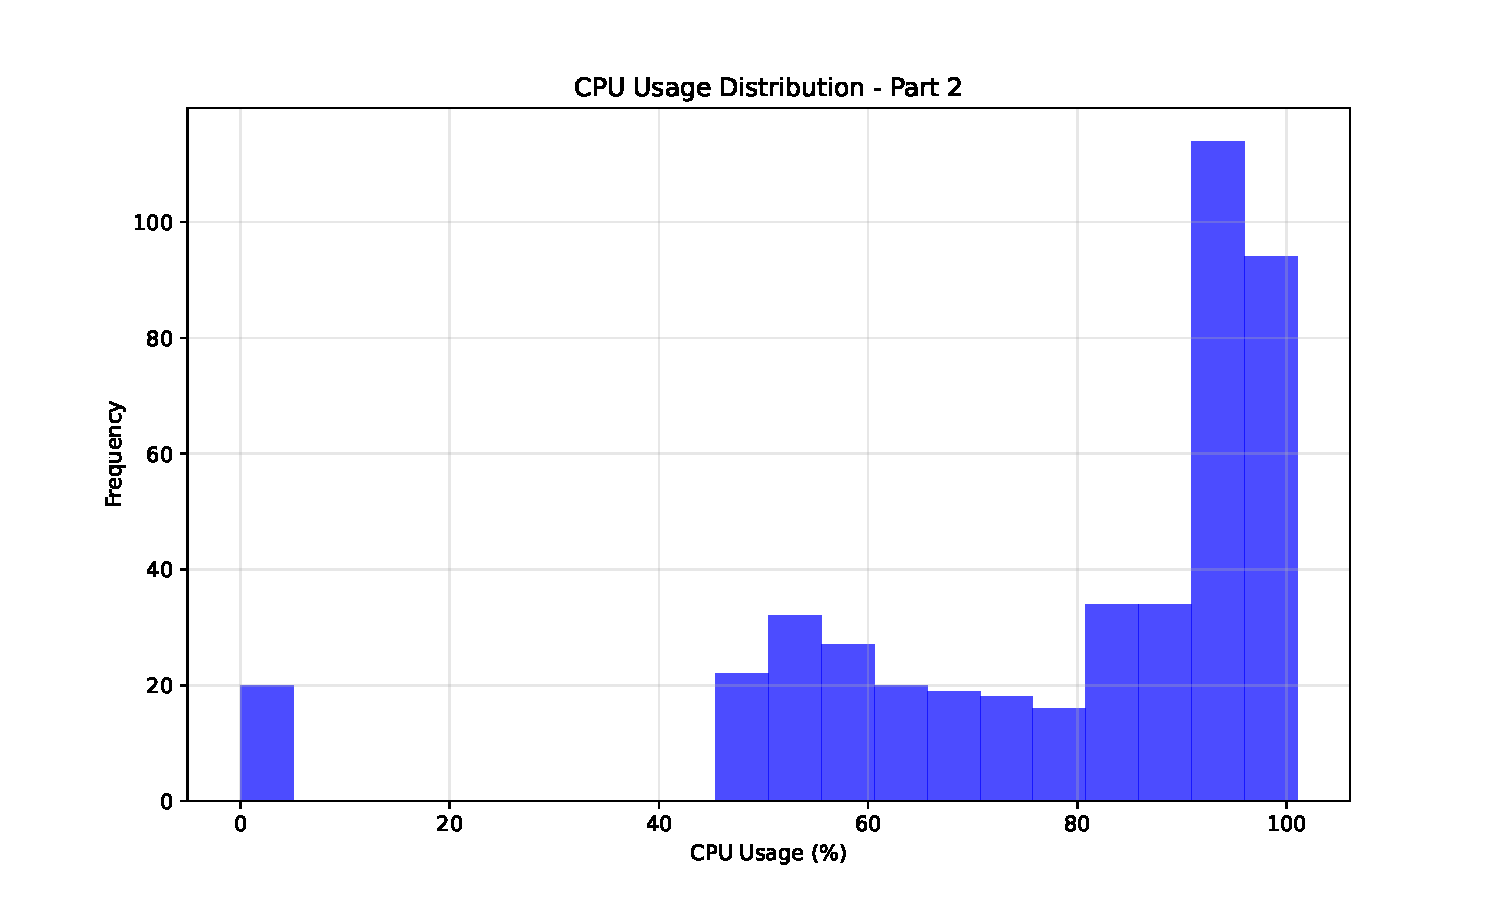
\includegraphics[width=0.8\textwidth]{figures/cpu_dist_part2.pdf}
    \caption{CPU usage distribution for N+1 processes on N cores}
    \label{fig:part2_cpu}
\end{figure}

\subsection{Part 3: Effect of Priority}

When one process was given a higher priority using \texttt{renice -n -10}, we observed that this process received more CPU time compared to other processes. The higher priority process consistently showed higher CPU usage percentages, demonstrating that CFS respects process priorities when allocating CPU time.

The nice value influences the "weight" calculation in CFS, which determines how much CPU time a process receives. Processes with lower nice values (higher priority) get more weight and consequently more CPU time. However, it's important to note that CFS still ensures that lower-priority processes receive some CPU time rather than being completely preempted.

\begin{figure}[H]
    \centering
    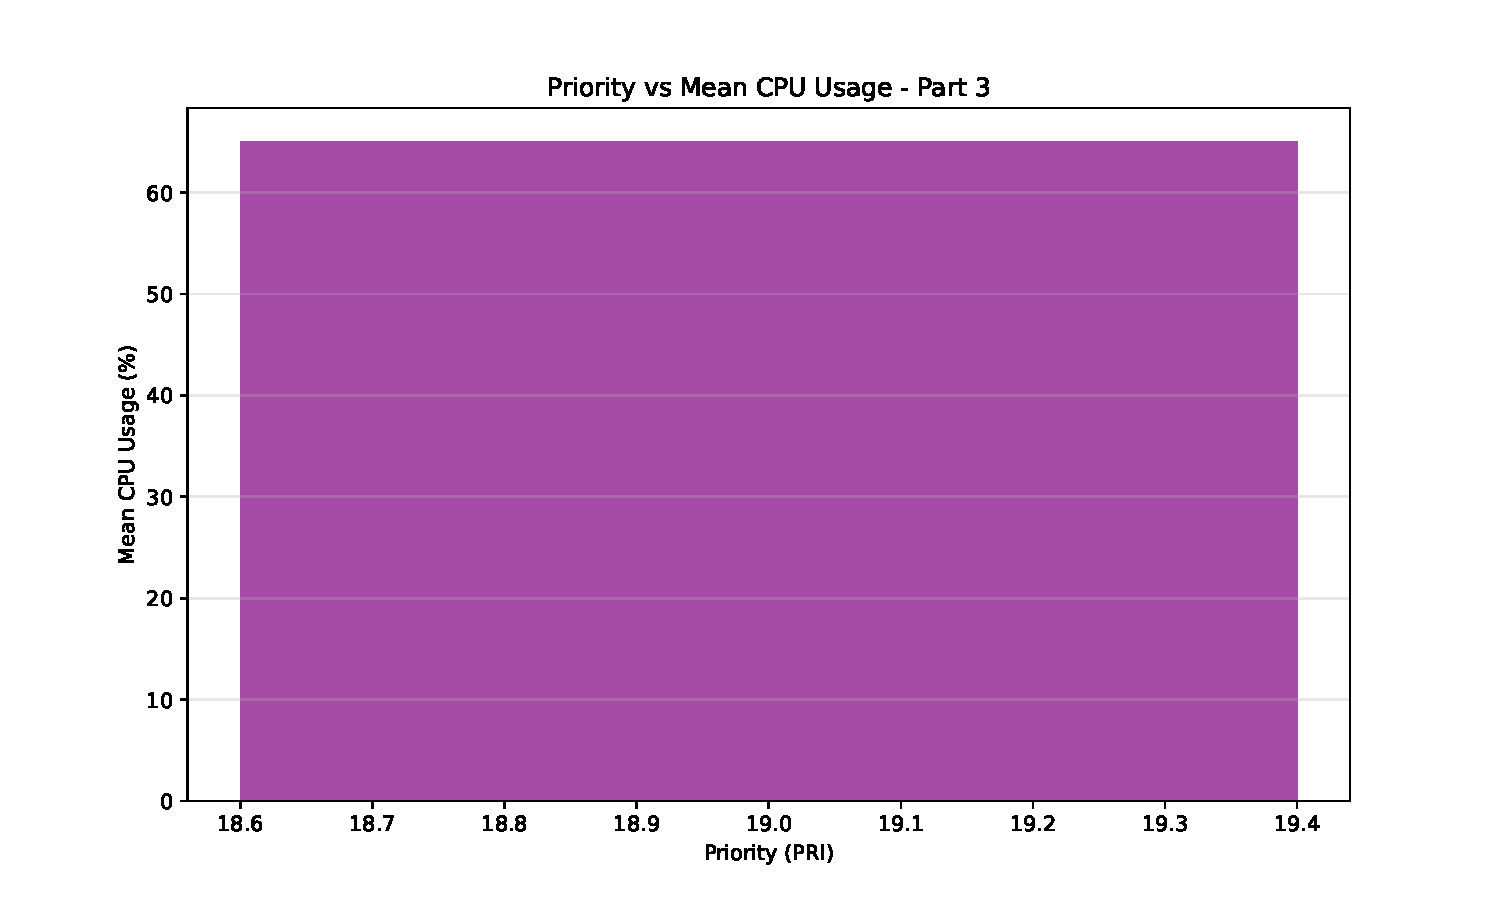
\includegraphics[width=0.8\textwidth]{figures/priority_cpu_part3.pdf}
    \caption{Priority vs. CPU usage for processes with different nice values}
    \label{fig:part3_priority}
\end{figure}

\subsection{Part 4: Process Blocked by Input}

When running N CPU-intensive processes and one process blocked waiting for input, we observed that the blocked process spent most of its time in the "S+" state (interruptible sleep in the foreground). While in this state, the process consumed negligible CPU resources.

When the blocked process received input, it briefly transitioned to the "R+" state, consumed some CPU time to process the input, and then returned to the "S+" state while waiting for more input. This behavior demonstrates how CFS efficiently handles I/O-bound processes, allowing them to respond promptly to I/O events without wasting CPU cycles while waiting.

\begin{figure}[H]
    \centering
    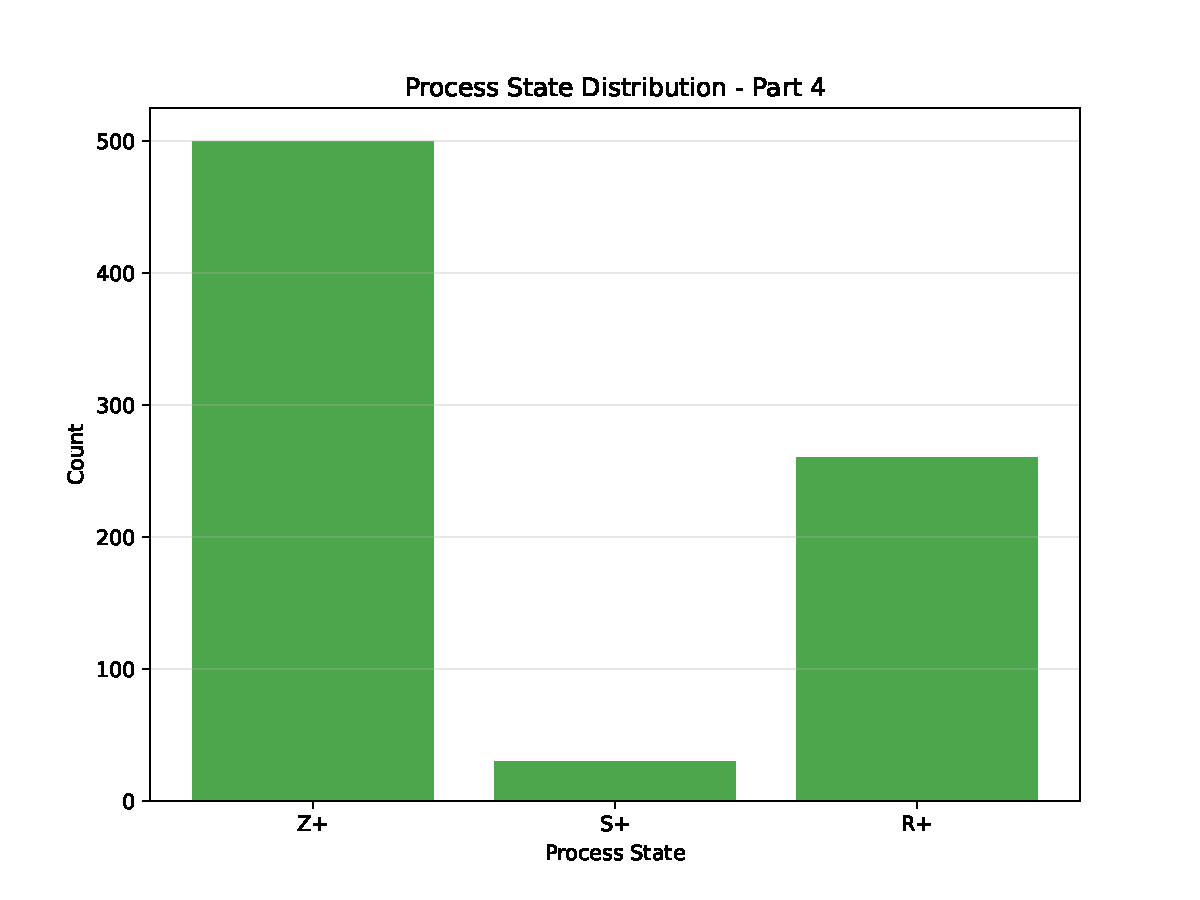
\includegraphics[width=0.8\textwidth]{figures/state_dist_part4.pdf}
    \caption{Process state distribution for N CPU-intensive processes + 1 I/O-bound process}
    \label{fig:part4_state}
\end{figure}

\section{Comparative Analysis}

\subsection{CFS vs. Other Scheduling Algorithms}

The Linux Completely Fair Scheduler shows several distinct characteristics compared to traditional scheduling algorithms:

\begin{table}[H]
\centering
\begin{tabular}{|p{2.5cm}|p{11cm}|}
\hline
\textbf{Scheduler} & \textbf{Characteristics} \\
\hline
CFS & Tracks virtual runtime for each process to ensure fairness. Processes with the least virtual runtime get scheduled next. Employs weighted fair queueing based on process priority. Uses a red-black tree for efficient process selection. \\
\hline
FIFO & Processes run in the order they arrive until completion. No preemption except for higher priority processes. Can lead to convoy effect where short processes wait behind long ones. \\
\hline
Round Robin & Allocates fixed time quantum to each process in a circular queue. Ensures every process gets CPU time but may lead to high context switching overhead. \\
\hline
SJF & Prioritizes processes with shortest execution time. Optimal for minimizing average waiting time but requires knowledge of process execution time in advance. Can lead to starvation of long processes. \\
\hline
\end{tabular}
\caption{Comparison of scheduling algorithms}
\label{tab:scheduler_comparison}
\end{table}

\subsection{CPU Distribution Analysis}

Our experiments revealed the following key observations about how CFS distributes CPU time:

\begin{enumerate}
    \item \textbf{Equal Resources}: When resources are sufficient (N processes on N cores), CFS allocates one core to each process.
    
    \item \textbf{Resource Contention}: When resources are insufficient (N+1 processes on N cores), CFS reduces the allocation for all processes rather than starving any one process.
    
    \item \textbf{Priority Influence}: Process priorities (nice values) influence the distribution of CPU time, with higher priority processes receiving more time.
    
    \item \textbf{Process Type Awareness}: I/O-bound processes are treated differently from CPU-bound processes, receiving prompt service when they need CPU time but not consuming resources while waiting.
\end{enumerate}

\section{Conclusion}

The Linux Completely Fair Scheduler lives up to its name by providing fair CPU time allocation among competing processes. Our experiments demonstrated several key aspects of CFS behavior:

\begin{enumerate}
    \item CFS efficiently distributes CPU resources when the number of processes equals the number of CPU cores.
    
    \item When processes exceed available cores, CFS maintains fairness by reducing the allocation for all processes rather than starving some.
    
    \item Process priorities influence CPU allocation, but CFS ensures that even low-priority processes receive some CPU time.
    
    \item CFS effectively handles the different needs of CPU-bound and I/O-bound processes.
\end{enumerate}

These characteristics make CFS well-suited for general-purpose computing environments where fairness, responsiveness, and efficient resource utilization are important. Compared to traditional algorithms like FIFO, Round Robin, or Shortest Job First, CFS offers a balanced approach that handles diverse workloads while maintaining fairness.

The virtual runtime tracking and weighted fair queueing mechanisms of CFS provide better overall system responsiveness than simpler algorithms, particularly in mixed workload scenarios with both CPU-intensive and interactive processes.

\appendix
\section{Code Implementation}

The experiments were implemented using C code that spawned processes and monitored their behavior. The implementation used system calls such as \texttt{fork()}, \texttt{exec()}, and process monitoring via the \texttt{ps} command.

Key components of the implementation included:

\begin{itemize}
    \item Process creation using \texttt{fork()} and custom task functions
    \item Process monitoring using \texttt{ps} command piped to log files
    \item Process priority adjustment using the \texttt{renice} command
    \item I/O-bound process simulation using a blocking read operation
\end{itemize}

\section{Analysis Methodology}

The analysis was performed using Python scripts that parsed the log files generated during the experiments. The analysis focused on:

\begin{itemize}
    \item CPU usage statistics (mean, median, standard deviation)
    \item Process state distributions
    \item Correlation between process priorities and CPU allocation
\end{itemize}

Statistical methods were used to analyze the data and generate visualizations that highlight the key behaviors of the Linux scheduler under different conditions.

\end{document}